\documentclass[a4paper, 11pt]{article}
\usepackage[polish]{babel}
\usepackage[MeX]{polski}
\usepackage[utf8]{inputenc}
\usepackage[T1]{fontenc}
%\usepackage{times}
\usepackage{graphicx,wrapfig}
%\usepackage{anysize}
%\usepackage{tikz}
%\usetikzlibrary{calc,through,backgrounds,positioning}
\usepackage{anysize}
\usepackage{float}
\usepackage{hyperref}
%\usepackage{stmaryrd}
%\usepackage{amssymb}
%\usepackage{amsthm}
%\marginsize{3cm}{3cm}{3cm}{3cm}
%\usepackage{amsmath}
%\usepackage{color}
%\usepackage{listings}
%\usepackage{enumerate}
%\lstloadlanguages{Ada,C++}


\begin{document}	
	% \noindent -  w tym akapicie nie bedzie wciecia
	% \ indent - to jest aut., ale powoduje ze jest wciecie
	% \begin{flushleft}, flushright, center - wyrownianie akapitu
	% \textbf{pogrubiany tekst}
	% \textit{kursywa} 
	% 					STRONY 
	%  http://www.codecogs.com/latex/eqneditor.php 
	%  http://www.matematyka.pl/latex.htm
	% 
	\begin{titlepage}
		
		
		
		\newcommand{\HRule}{\rule{\linewidth}{0.5mm}} % Defines a new command for the horizontal lines, change thickness here
		
		\center % Center everything on the page
		
		%----------------------------------------------------------------------------------------
		%	HEADING SECTIONS
		%----------------------------------------------------------------------------------------
		
		\textsc{\LARGE Akademia Górniczo-Hutnicza im. Stanisława Staszica}\\[1.5cm] % Name of your university/college
		\textsc{\Large Kraków}\\[0.5cm] % Major heading such as course name
		\textsc{\large }\\[0.5cm] % Minor heading such as course title
		
		%----------------------------------------------------------------------------------------
		%	TITLE SECTION
		%----------------------------------------------------------------------------------------
		
		\HRule \\[0.4cm]
		{\fontsize{38}{50}\selectfont Symulator pożaru lasu}
		%	{ \Huge \bfseries} Symulator pożaru lasu\\[0.3cm] % Title of your document
		\HRule \\[1.5cm]
		
		%----------------------------------------------------------------------------------------
		%	AUTHOR SECTION
		%----------------------------------------------------------------------------------------
		
		% If you don't want a supervisor, uncomment the two lines below and remove the section above
		\Large \emph{Autorzy:}\\
		Sebastian \textsc{Katszer}\\ % Your name
		Katarzyna \textsc{Kosiak} \\[3cm]\ % Your name
		
		
		%----------------------------------------------------------------------------------------
		%	DATE SECTION
		%----------------------------------------------------------------------------------------
		
		{\large \today}\\[3cm] % Date, change the \today to a set date if you want to be precise
		
		%----------------------------------------------------------------------------------------
		%	LOGO SECTION
		%----------------------------------------------------------------------------------------
		
		%\includegraphics{Logo}\\[1cm] % Include a department/university logo - this will require the graphicx package
		
		%----------------------------------------------------------------------------------------
		
		\vfill % Fill the rest of the page with whitespace
		
	\end{titlepage}
	
	%SPIS TRESI
	%
	%
	%
	%
	%
	%
	%
	%
	%
	
	\vfill
	\newpage
	%\pagebreak
	
	%SEKCJE
	%opis zagadnienia, temat, problem, dlaczego chcemy to rozwiązacyać metodą ewolucyjnę
	%jakie są metody rozwiącania problemu, przegląd literatury,
	%proponowane rozwiązania (spójność)
	%czym się inspierowałyśmy
	%
	%
	%
	
	%\setlength{\parskip}{1ex plus 0.5ex minus 0.2ex}
	
	\section{Wstęp}
	\indent
	
	Niniejszy dokument stanowi specyfikację programu do symulowania pożarów lasów, który został stworzony na potrzeby przedmiotu ''Modelowanie i symulacja systemów'' i rozbudowany na potrzeby przedmiotu ''Studio projektowe 2''.
	
	\section{Funkcjonalność aplikacji}
	\indent
	
	Program przyjmuje dane wejściowe od użytownika i uruchamia symulację pożaru. Jest też możliwość uruchomienia wgranego, przykładowego pożaru bazowanego na początkowych etapach pożaru Kuźni Raciborskiej w 1992 roku. \\
	
	Dane wejściowe wprowadzane przez użytkownika podzielone są na sekcje: 
		\begin{itemize}
			\item Teren - długości boków terenu, nierówność terenu, maksymalna wysokość.
			\item Roślinność - trzy poziomy gęstości zalesienia (rzadki, zwykły, gęsty), trzy rodzaje lasów (liściasty, iglasty i mieszany).
			\item Pogoda - prędkość wiatru, kierunek wiatru, wilgotność powietrza.
			\item Szybkość symulacji.
		\end{itemize}
		\begin{figure}[H]
			\centerline{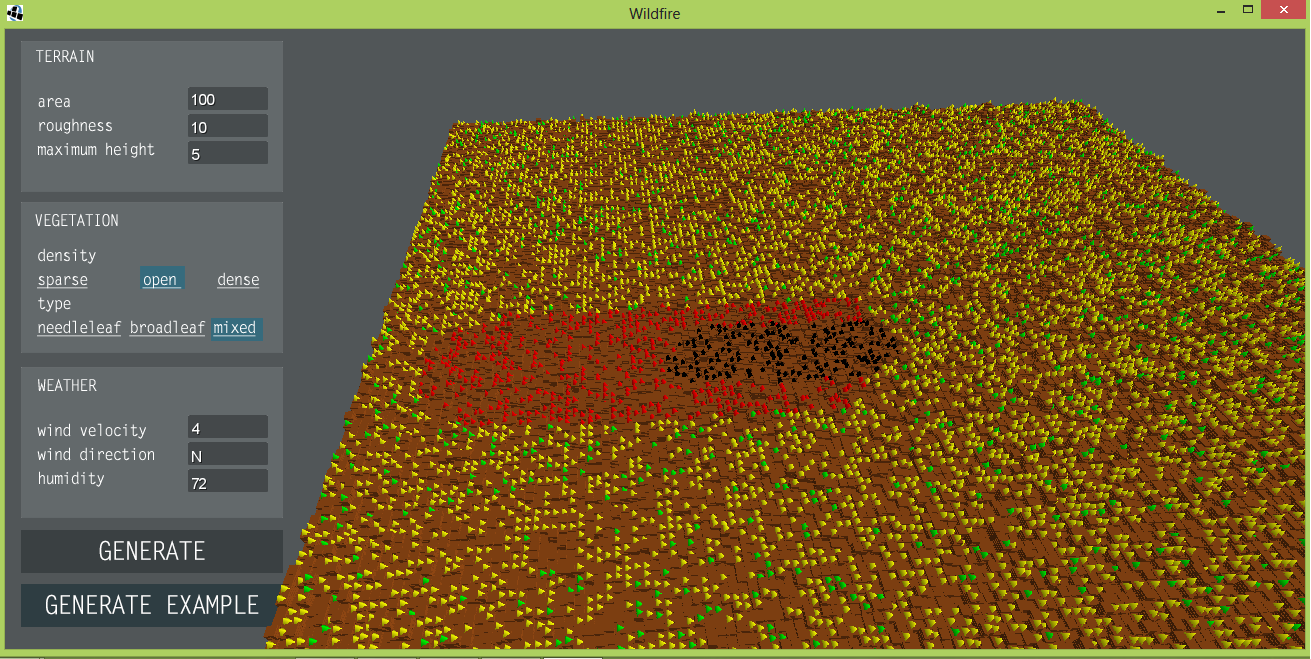
\includegraphics[scale=0.4]{pictures/gui1.png}}
		\end{figure}
		
	Model wykorzystuje automaty komórkowe i model Rothermela do symulowania przebiegu pożaru. Linia ognia przybiera kształt eliptyczny i mają na nią wpływ wszystkie zadane przez użytkownika dane poza wilgotnością powietrza oraz nachyleniem stoku. Drzewa mają różny czas zapłonu w zależności od gatunku.
	
	Trójwymiarowy model terenu można obracać w trakcie trwania symulacji. Po zakończeniu symulacji wyświetlany jest krótki raport informujący o czasie symulacji, ilości wszystkich drzew, ilości i procencie spalonych i żywych drzew. 
	
	\section{Diagramy UML}
	\indent
	
	Ze względu na duże wymiary plików z diagramami klas, nie zostały one włączone do tego dokumentu. Diagramy klas znajdują się w załączonym folderze o nazwie pictures. Znajdują się w nim: \\
	
	\begin{itemize}
		\item simulation -- Główna paczka odpowiedzialna za logiczną sferę symulacji		
		\item data -- Zawiera dane i stałe, na których bazuje symulacja, mogą być one aktualizowane podczas symulacji.
		\item graphic -- Paczka ta zawiera klasy odpowiedzialne za wizualną stronę aplikacji.
		\item model -- Przechowuje wykorzystywane abstrakcyjne modele odzwierciedlające rzeczywistość.
	\end{itemize}
	
	\section{Zarządzanie projektem}
	\indent
	
	W początkowych fazach projektu w rozporządzaniu zadaniami pomagała nam webowa aplikacja Trello oparta na tablicy kanban. Mimo przyjaznego interfejsu, z powodu zbyt małej elastyczności aplikacji przenieśliśmy się na inną webową aplikację - MeisterTask. Spełnia ona nasze oczekiwania dotyczące przejrzystości interfejsu i rozporządzania zadaniami w czasie. \\
	\begin{figure}[H]
		\centerline{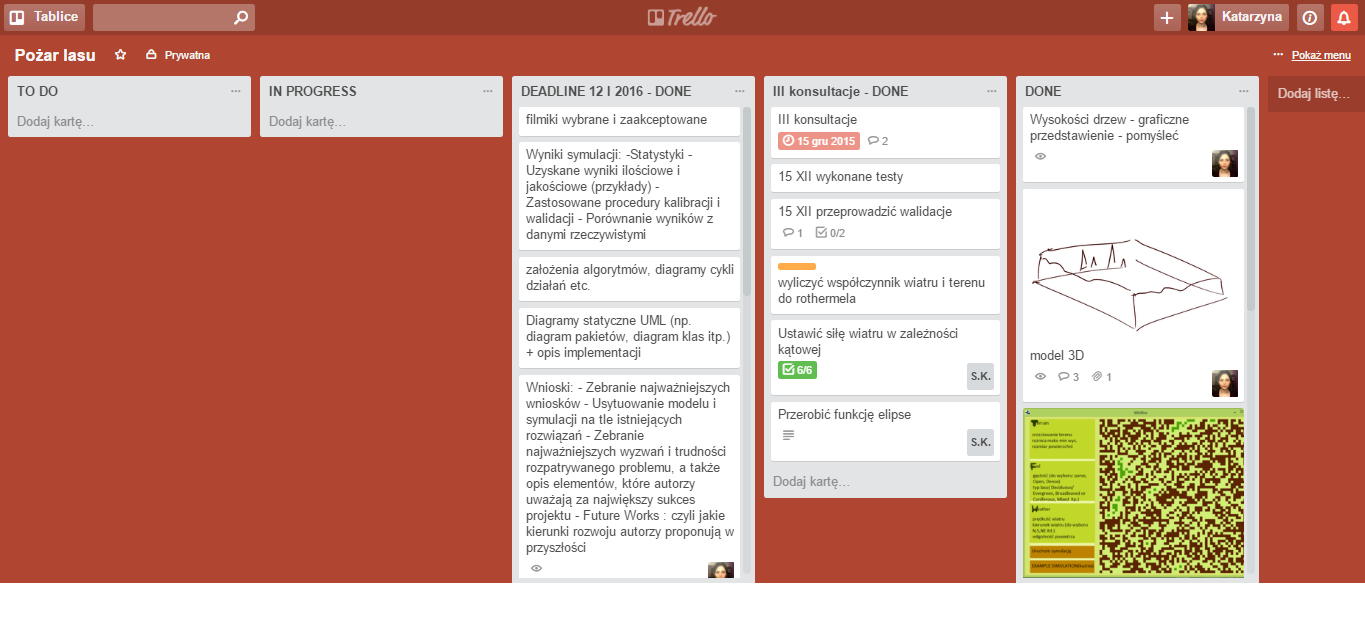
\includegraphics[scale=0.4]{pictures/trello.png}}
		\raggedright{	\caption{Przykładowy stan naszego projektu na Trello}}
	\end{figure}
	\begin{figure}[H]
		\centerline{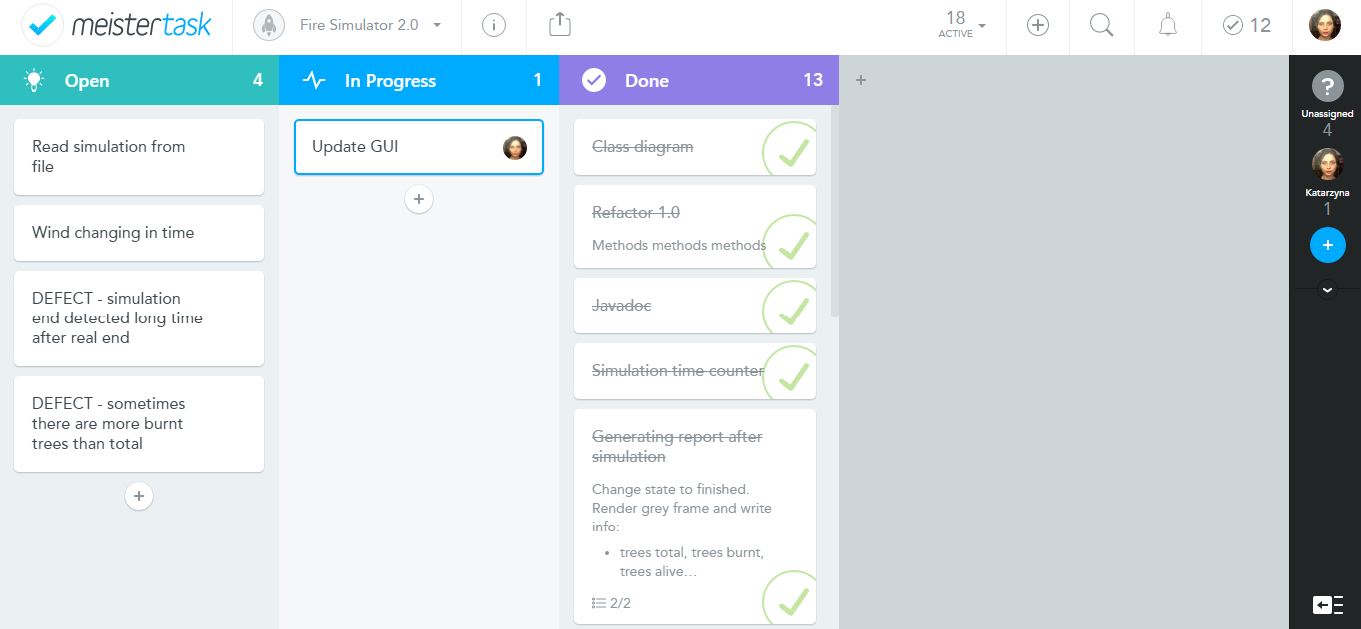
\includegraphics[scale=0.4]{pictures/meister.png}}
		\raggedright{	\caption{Przykładowy stan naszego projektu na MeisterTask}}
	\end{figure}
	
	\section{Krótki opis poszczególnych klas}
	\indent
	
		\begin{itemize}
			\item GraphicController - kontroluje wyświetlanie odpowiednich elementów GUI, obsługuje akcje użytkownika, zarządza wyświetlaniem symulacji i raportu.
			\item GraphicUtils - jest zbiorem dodatkowych metod przydatnych przy wyświetlaniu wewnętrznych danych w odpowiedniej formie i wykrywaniu akcji użytkownika.
			\item Models - zawiera i inicjalizuje trójwymiarowe modele dla celów symulacji.
			\item Textures - zawiera i inicjalizuje tekstury dla interfejsu użytkownika.
			\item Simulation - posiada ogólne informacje o symulacji i jej przebiegu, np. czas rozpoczęcia.
			\item Cell - jest najmniejszym elementem (komórką automatu) znajdującym się na symulowanym terenie. Reprezentuje roślinność i posiada swój stan.
			\item Terrain - jest zbiorem komórek i posiada metody odpowiadające za przebieg pożaru.
			\item Data - zbiór szczegółowych danych aktualnej symulacji oraz przykładowej symulacji pożaru Kuźni Raciborskiej.
		\end{itemize}
		
	
	\section{Szczegółowy opis metod klas}
	\indent
	
	Na stronie \url{http://student.agh.edu.pl/~kosiak/wildfireDocumentation/} znajduje się dokumentacja wygenerowana przy pomocy Javadoca. Zawiera ona krótkie opisy istotnych metod i podsumowanie funcjonalności wszystkich klas.

\end{document}
